\subsubsection{Dynamic Compression}
\label{sec:compression}

Compression selectively regulates the amplitudes of the audio output when they
exceed above the given threshold, making only these selected portions sound quieter.
In other words, compression reduces the dynamic range of the audio signal, therefore
balancing the loud and quiet parts of the audio. The following factors determine
the behavior of the compressor \cite{dutilleux_nonlinear2011}:

\begin{itemize}
    \item \textbf{Threshold:} The level (in dB) above which the compressor starts reducing the gain of the audio signal.
    Any audio signal below this threshold remains unaffected.
    \item \textbf{Ratio:} The factor of gain reduction applied to the audio signal that exceeds the threshold.
    For example, a ratio of 4:1 means that for every 4 dB above the threshold, the output will only decrease to 1 dB.
    \item \textbf{Attack Time:} The speed at which the compressor responds after the threshold is crossed. 
    A shorter attack time results in a faster response, while a longer attack time allows more of the initial transient to pass through.
    \item \textbf{Release Time:} The speed at which the compressor stops reducing the gain after the audio signal falls below the threshold.
\end{itemize}

\Cref{fig:comp_flowchart} presents a flowchart of the dynamic compression algorithm, which illustrates
the steps involved in processing the audio signal and applying gain reduction based on the threshold, 
ratio, attack time, and release time.

\begin{figure}[ht]
  \centering
  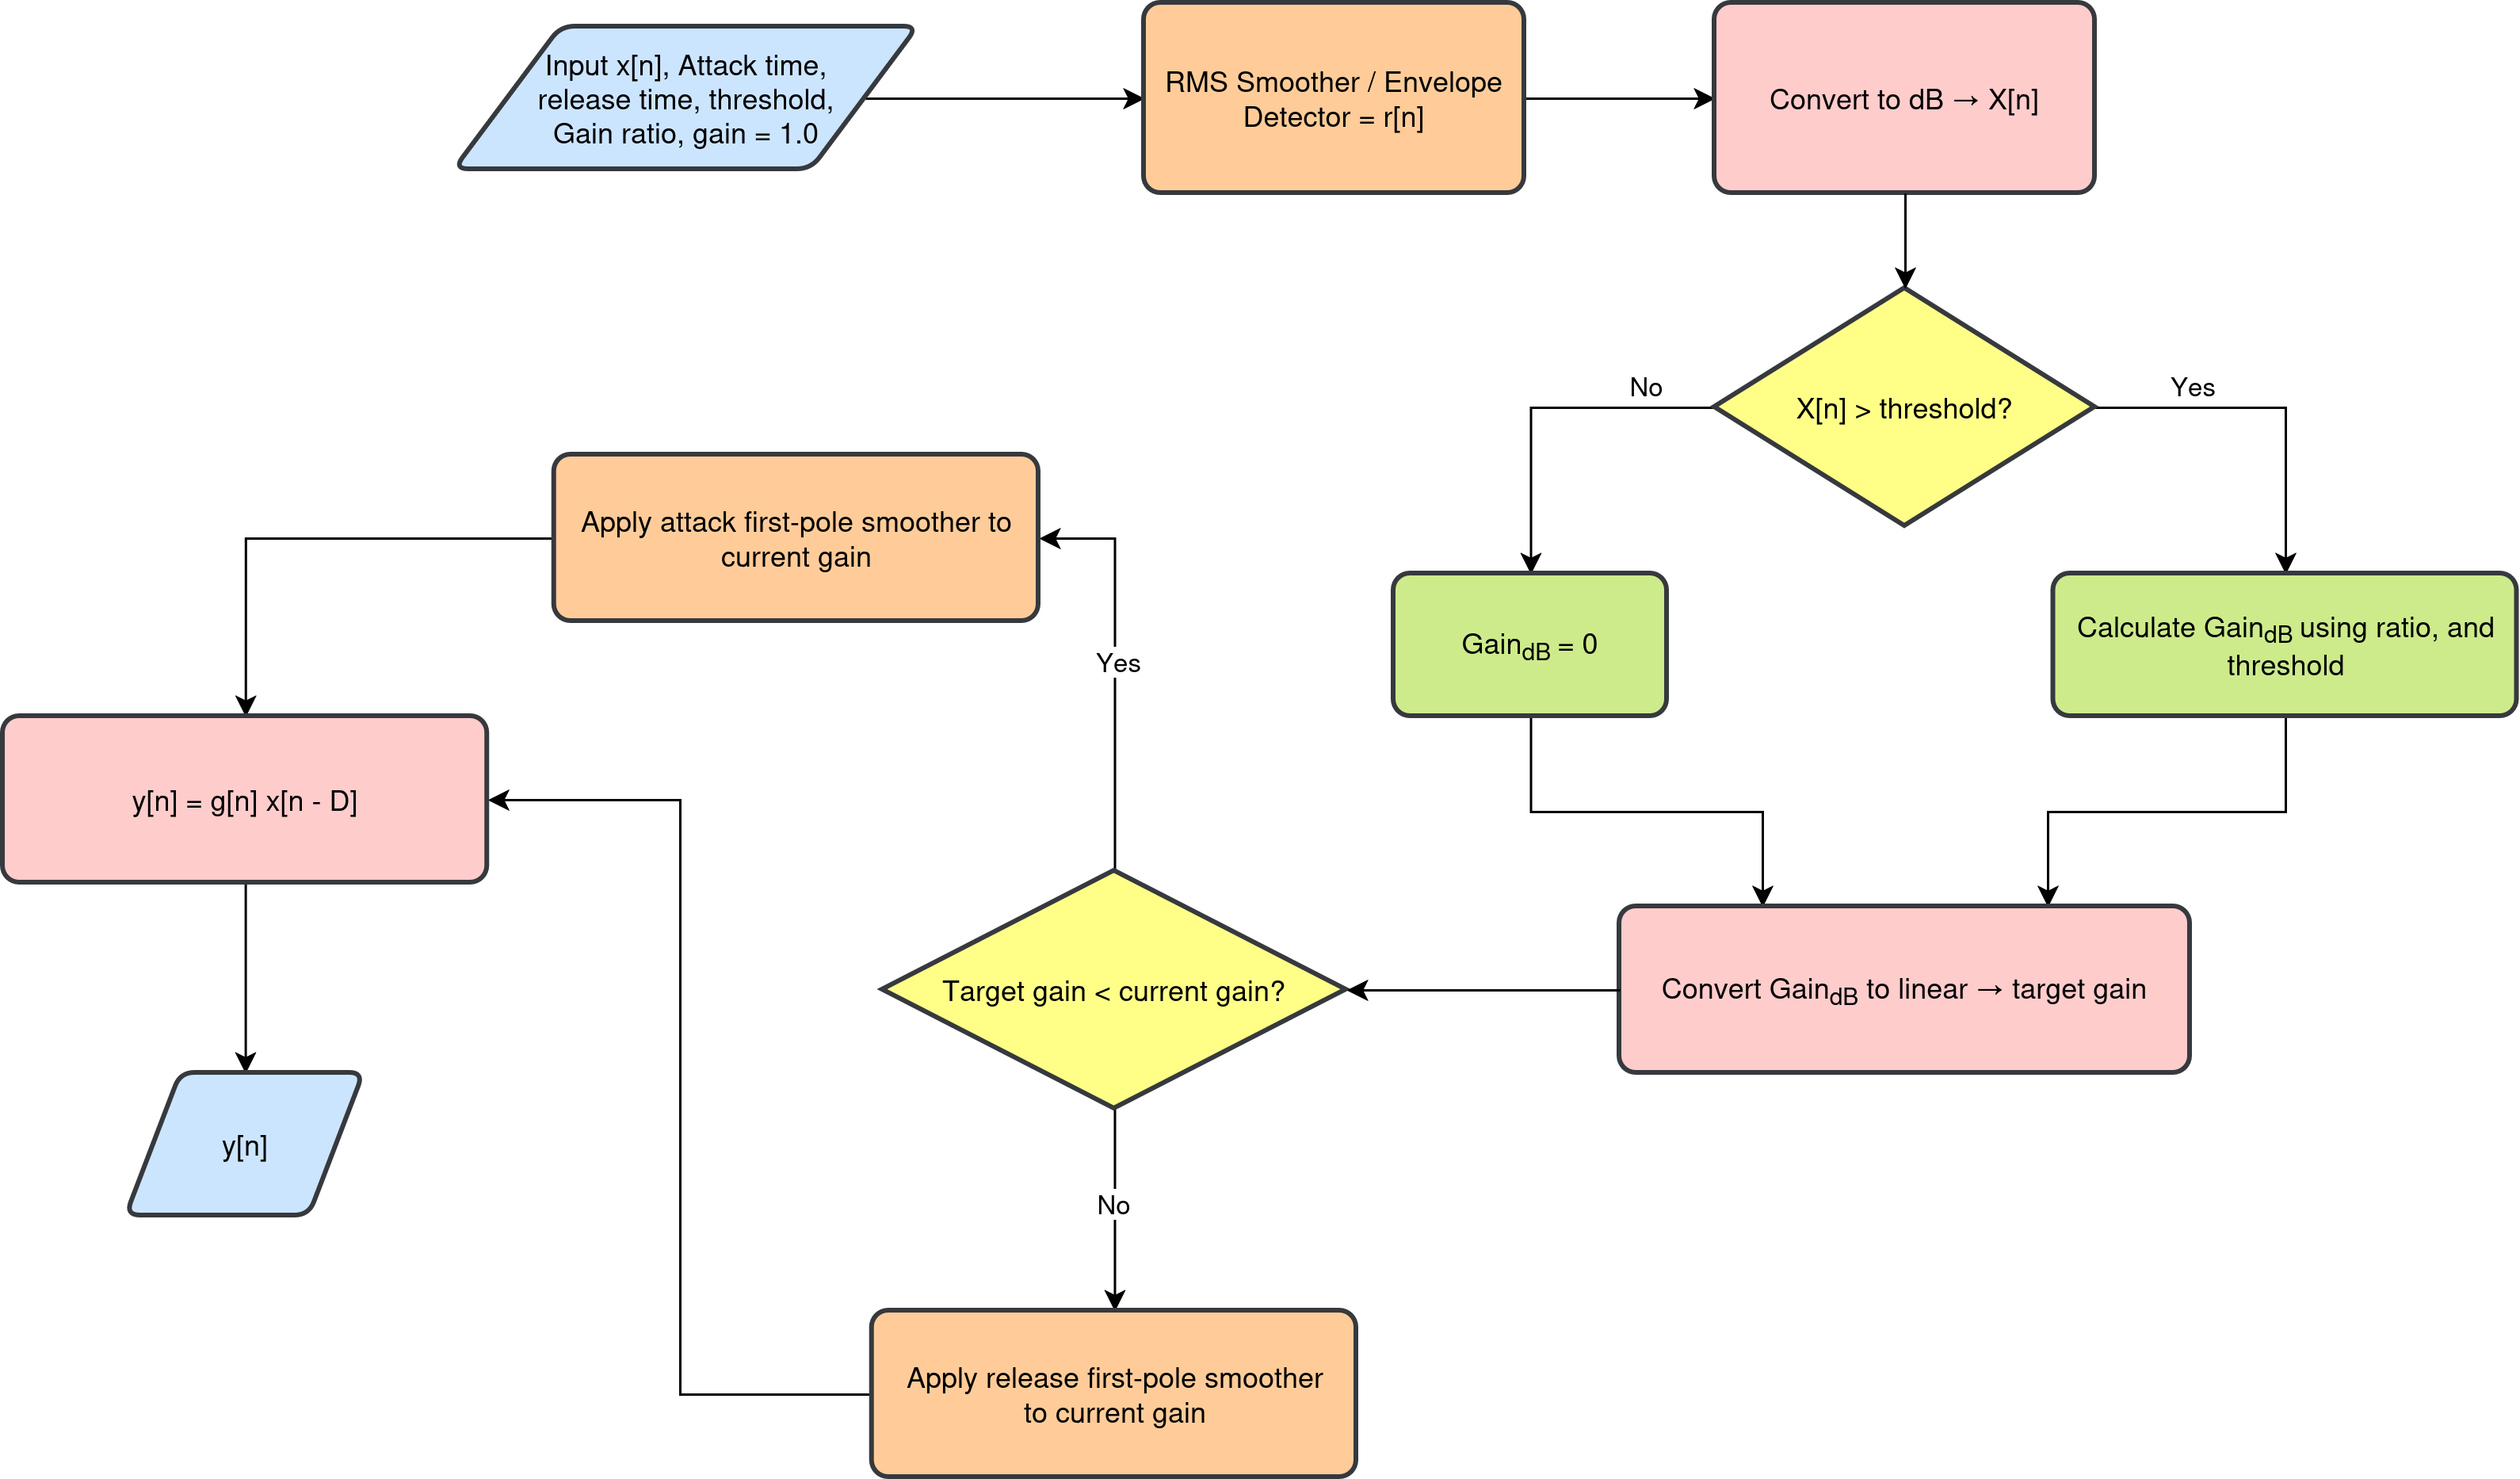
\includegraphics[width=\linewidth]{discussion/audio_effects/compression/figures/Compressor Flowchart.drawio.png}
  \caption{Flowchart illustrating the algorithm behind compression}
  \label{fig:comp_flowchart}
\end{figure}

To achieve this algorithm (\Cref{prompt:compressor_algorithm}) \cite{dutilleux_nonlinear2011,anthropicclaude}, 
the attack times, release times, and the RMS times are converted
to coefficients using the following equation with input $x[n]$, derived from envelope detection:

\begin{equation}\label{eq:time_to_coef}
    \alpha = 1 - e^\frac{-2.2}{tf_s}
\end{equation}

Where $t$ is either the attack times or release times, whichever is applied. These coefficients
determine how quickly the compression responds.

The following a recursive one-pole smoother is applied, described
using this equation:

\begin{equation}\label{eq:first_smoother}
    r[n] = (1 - \alpha_{rms}) r[n-1] + \alpha_{rms} x^2 [n]
\end{equation}

Which is then converted to decibels:
\begin{equation}\label{eq:X_decibels}
    X[n] = 10 \log_{10}(r[n] + \varepsilon), \qquad \varepsilon = 1 \times 10^{12}
\end{equation}

Note that $\varepsilon$ is applied to explicitly avoid $\log_{10}(0) = -\infty$, whenever the signal is silent.

With the level, $X[n]$ from \eqref{eq:X_decibels}, the given threshold $X_T$, and a ratio $R : 1$,
the gain compression curve is defined conditionally to leave signals below the threshold ($X[n] \le X_T$) 
unchanged:
\begin{equation}\label{eq:gain_equation}
    G[n] =
    \begin{cases}
        0, & X[n] \le X_T \\
        -\left(1 - \frac{1}{R} \right) \left( X[n] - X_T \right), & X[n] > X_T
    \end{cases}
\end{equation}

Which is then changed to linear, and used as target gain $g_{\text{target}}$:
\begin{equation}\label{eq:gain_linear_target}
    g_{\text{target}}[n] = 10^\frac{G[n]}{20}
\end{equation}


With the $g_{\text{target}}$ set up from \eqref{eq:gain_linear_target}, if 
$g_{\text{target}} < g$, this indicates that more compression is needed, therefore the
attack coefficient is used, and vice versa for the release coefficient. Therefore,

\begin{equation}\label{eq:attack_or_release}
    \alpha =
    \begin{cases}
        \alpha_{AT}, & g_{\text{target}} < g \\
        \alpha_{RL}, & \text{otherwise}
    \end{cases}
\end{equation}

Moreover, the calculated gain cannot be applied instantly, otherwise the compressor
would produce clicks and distortion. Therefore, another one-pole smoother is implemented,
which comprises the following equation:
\begin{equation}\label{eq:second_smoother}
    g[n] = (1 - \alpha)g[n-1] + \alpha g_{\text{target}}[n]
\end{equation}

And finally, this dyanmically adjusting gain is applied, with optional delay, with $D$ as the lookahead delay in samples.
\begin{equation}\label{eq:compression_transfer}
    y[n] = g[n] x[n - D] 
\end{equation}

The code implementation of this algorithm above is provided in \Cref{app:compressor_Code}.

The following plot (\Cref{fig:compressor_plot}) shows an input sine wave with amplitude of 0.2, and changes to 0.8 at 1 second, 
and falls back to 0.2 at 2 seconds. The compressor is set with a threshold of -6 dB, a ratio of 4:1,
an attack time of 10 ms, and a release time of 100 ms. The averaging time TAV 
\cite{dutilleux_nonlinear2011} is set to 10 ms, and the lookahead delay is set to 150 samples. 

\begin{figure}[ht]
  \centering
  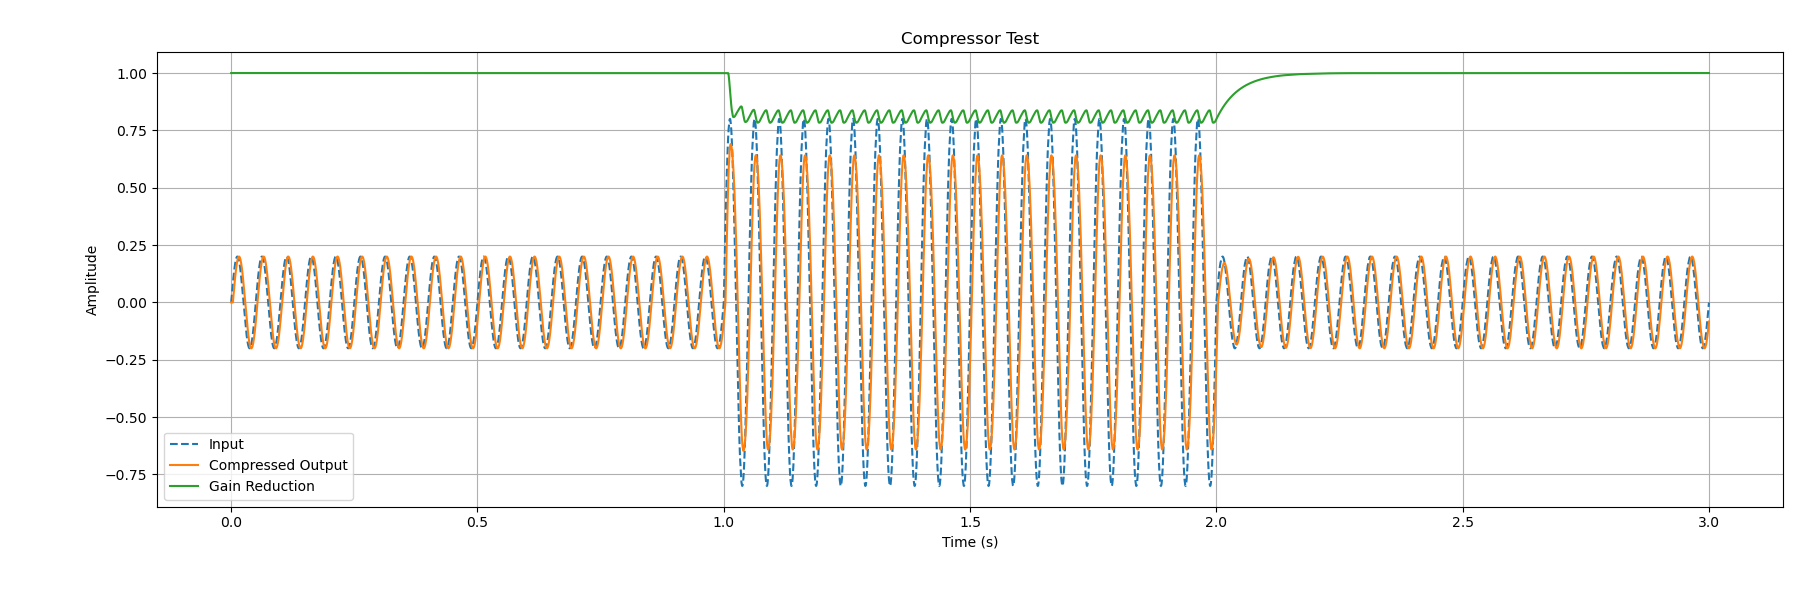
\includegraphics[width=\linewidth]{discussion/audio_effects/compression/figures/compressor_plot.png}
  \caption{Plot showing the effect of compression on the input signal with gain reduction applied}
  \label{fig:compressor_plot}
\end{figure}

The output shows the effect of compression on the input signal, with the gain reduction 
applied, and it provided expected results, as shown in \Cref{fig:compressor_plot}. However,
the gain reduction dropped from 1 to 0.79 (\SI{0}{\decibel} to \SI{-1.95}{\decibel}), and the RMS
values for the input and output signals are measured to be -4.94843 and -6.79832 dB respectively.
To check if the compressor is working correctly, the system confirms that it responds, since
$-4.94843 \text{dB} > -6.0 \text{dB}$. Therefore,

$$
\Delta \text{RMS}_\text{threshold} = -4.94843 \text{dB} - (-6.0 \text{dB}) = 1.05157 \text{dB}
$$

4:1 compression ratio means that any signal past -6 dB will be reduced to a quarter of its original amplitude in 
decibels \cite{pluginboutique_compression_guide}. Therefore, the change in RMS should be:
$$
\Delta \text{RMS}_\text{compression} = \frac{1}{4} \Delta \text{RMS}_\text{threshold} = \frac{1}{4} \times 1.05157 \text{dB} \\
= 0.26289 \text{dB}
$$

Therefore, the output level should be,
$$
y_\text{dB} = -6.0 \text{dB} + 0.26289 \text{dB} = -5.73711 \text{dB}
$$

However, the output level is measured to be \SI{-6.79832}{\decibel}, which is lower than the expected value of \SI{-5.73711}{\decibel}.
This discrepancy can perhaps be due to low attack times, which makes the compressor respond much faster and apply gain reduction to
higher amount.

Moreover, \Cref{fig:compressor_plot_high_att} shows the response of the output signal and gain reduction 
when the attack time is changed to 200 ms. All other parameters remain the same.

\begin{figure}[ht]
  \centering
  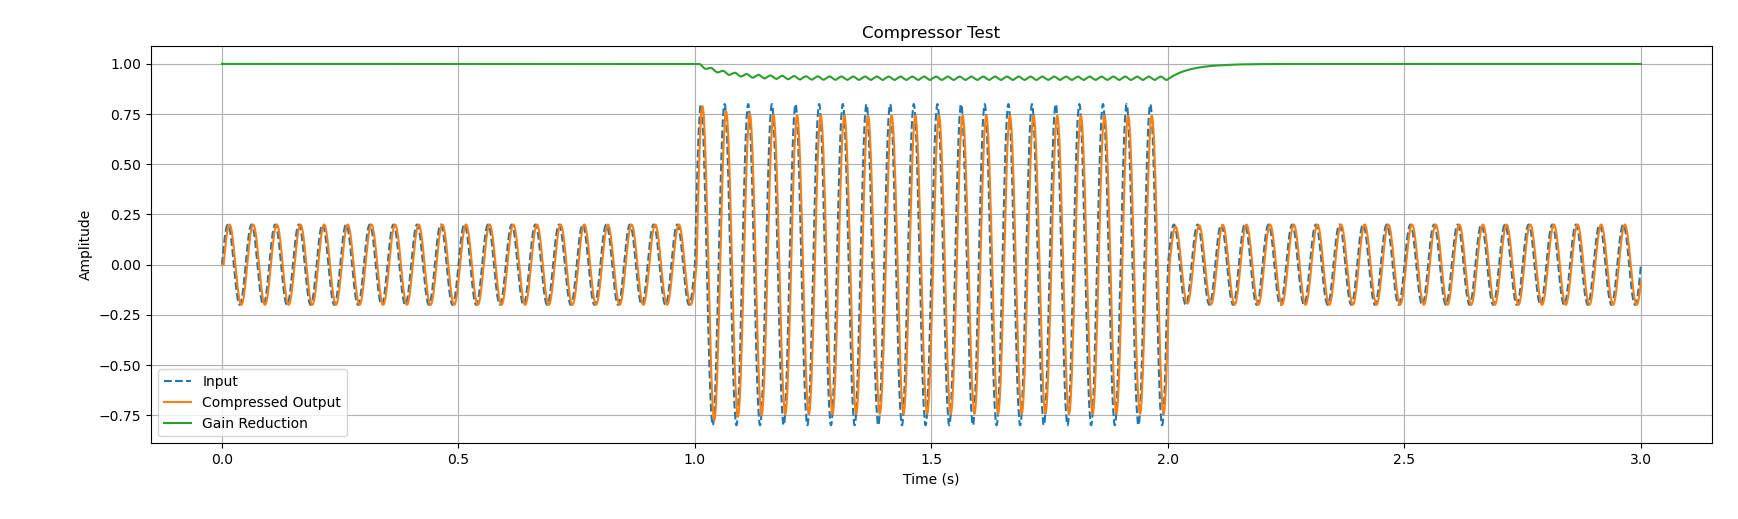
\includegraphics[width=\linewidth]{discussion/audio_effects/compression/figures/Compressor_plot_high_attack_time.png}
  \caption{Plot showing the effect of compression on the input signal as in \Cref{fig:compressor_plot}
  with an attack time of 200 ms}
  \label{fig:compressor_plot_high_att}
\end{figure}

It is observed that the gain reduction is less significant compared to the case with a shorter attack time 
(\SI{10}{\milli\second}), thus, making the compressor respond slower to the input signal. Also, the difference between 
the RMS values have reduced since the output is \SI{-5.55199}{\decibel}. This shows that the gain reduction and 
the transient response of the compressor might be sensitive to the attack time.

Therefore, with all these observations, it can be assumed that the compressor is working correctly, since it is 
known that it can respond to the input signal, and apply gain reduction, as expected.


